\chapter{Appendix: Swarmalators on an ER Network}
We now explore how the active phase wave state ($K = -0.6$, $J = 0.9$) behaves on an Erdős-Rényi (ER) network as the connection probability $p$ increases.

\section{Order Parameters}
A useful way to assess the system's state is through three order parameters \cite{O_Keeffe_2017}, independent of the network topology:
\begin{itemize}
    \item \( r \) measures the degree of phase synchronization, ranging from 0 (desynchronized) to 1 (fully synchronized), as introduced in the Kuramoto model \cite{Acebron_2005}:
    \begin{equation}
        r = \left| \frac{1}{N} \sum_{j=1}^{N} e^{i \theta_j} \right|
        \label{equation::r}
    \end{equation}
    \item \( S \) quantifies the correlation between phases \( \theta_j \) and spatial angles \( \phi_j \):
    \begin{equation}
        S = \max \left\{  \left| \frac{1}{N} \sum_{j=1}^{N} e^{i (\phi_j+\theta_j)} \right|, \left| \frac{1}{N} \sum_{j=1}^{N} e^{i (\phi_j-\theta_j)} \right| \right\}
        \label{equation::S}
    \end{equation}
    \item \( U \) measures the fraction of swarmalators that complete at least one full cycle in both space and phase:
    \begin{equation}
        U = \frac{N_{rot}}{N}
        \label{equation::U}
    \end{equation}
\end{itemize}
\( S \) is positive in both splintered and active phase wave states, while \( U \) is non-zero only in the active phase wave.

\newpage
\section{ER Network}
Using tools from the third laboratory, we implemented functions to compute the order parameters for each simulation. After reaching the steady state ($t_f = 300$), we computed \( r \), \( S \) (discarding the transient dynamics), and \( U \). Each value of $p$ was averaged over ten different realizations of the system to obtain means and standard deviations.

The results for $S$ and $U$ are shown below.

\begin{figure}[h]
    \centering
    \begin{minipage}[c]{0.8\textwidth}
        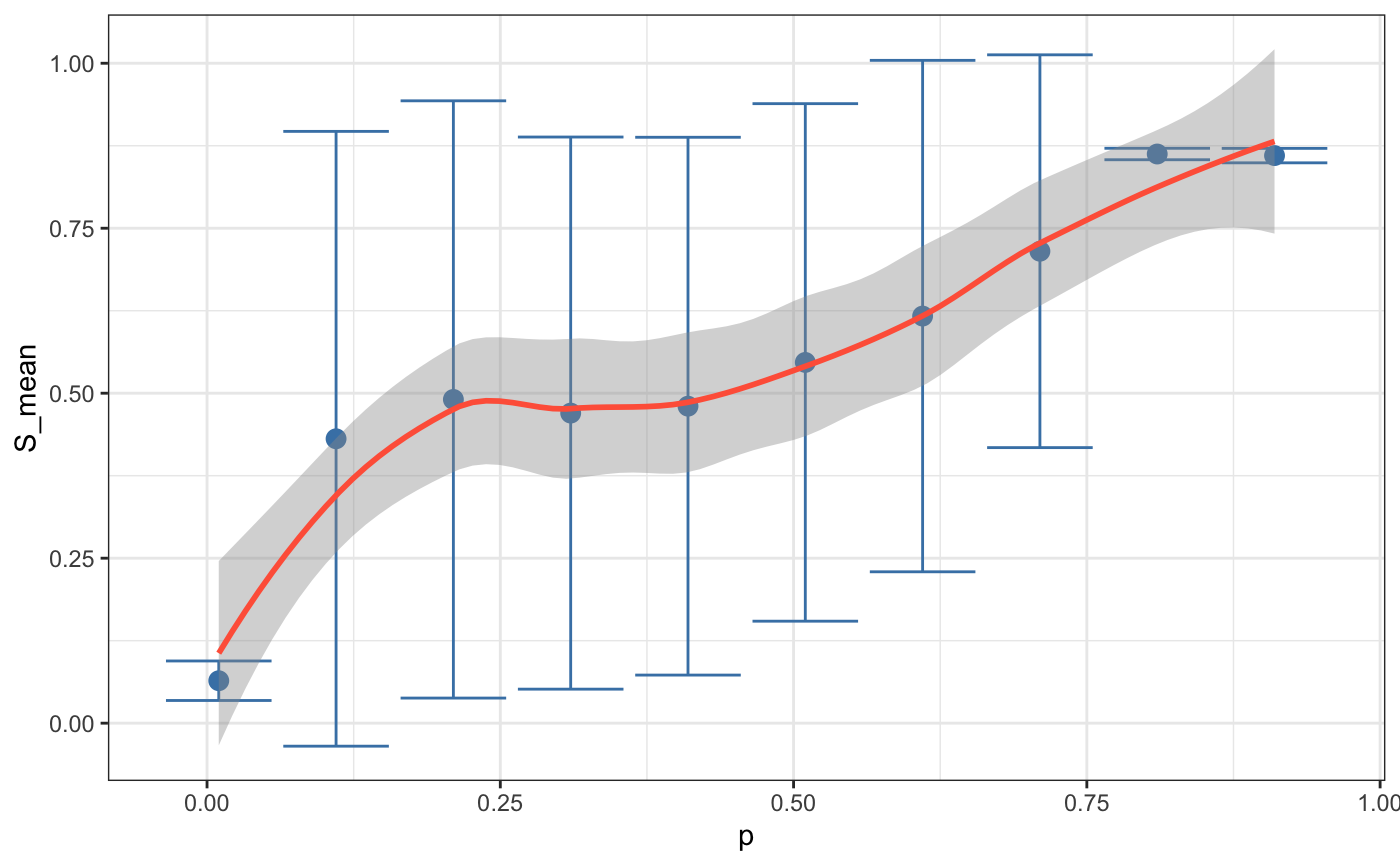
\includegraphics[width=\textwidth]{images/task1-appendix/S_K=-0.6,J=0.9.png}
    \end{minipage}
    \label{fig:S}
\end{figure}

\begin{figure}[h]
    \centering
    \begin{minipage}[c]{0.8\textwidth}
        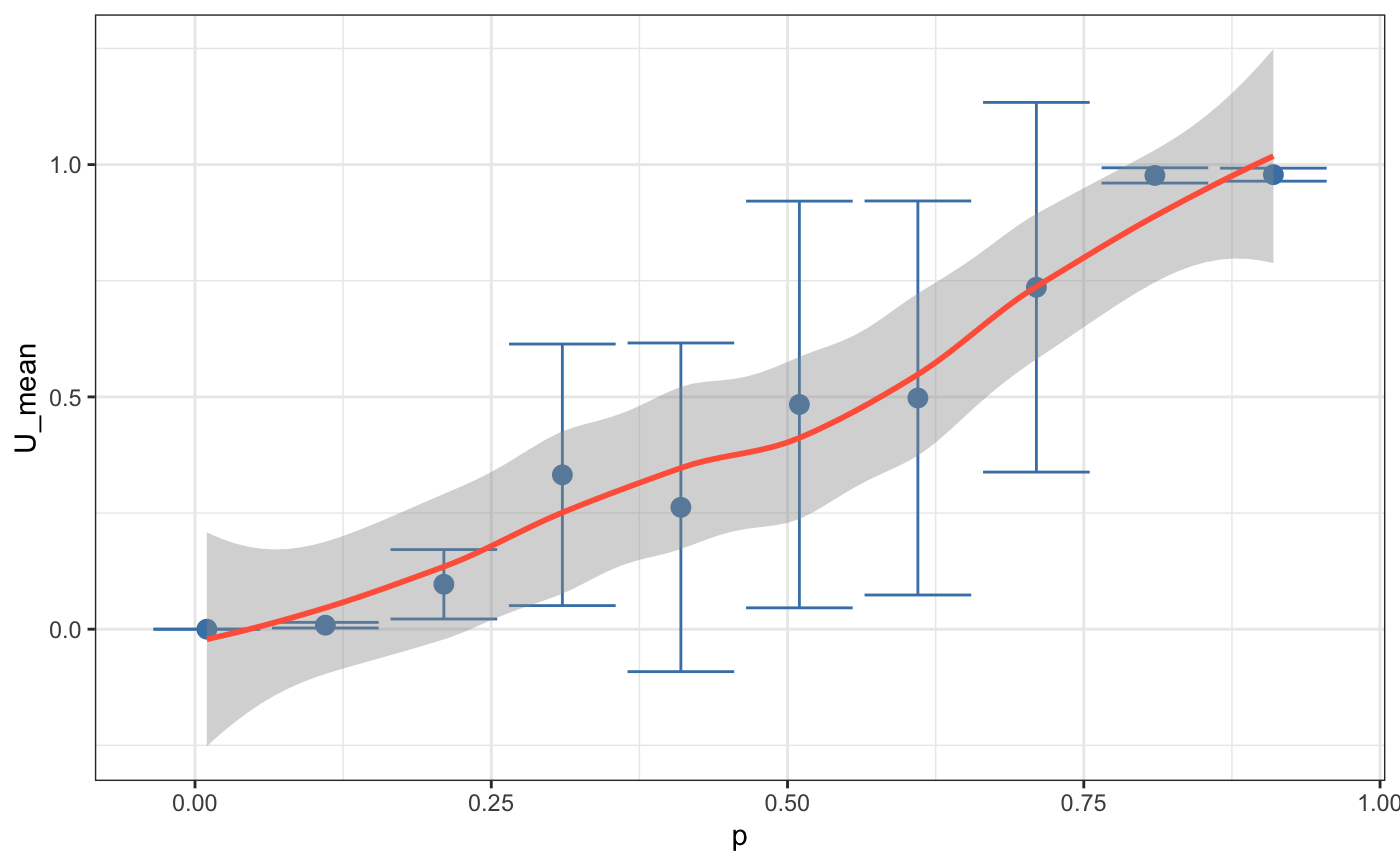
\includegraphics[width=\textwidth]{images/task1-appendix/U_K=-0.6,J=0.9.png}
    \end{minipage}
    \label{fig:U}
\end{figure}

Both $S$ and $U$ increase monotonically with $p$. 
It's possible that, as connectivity increases, more swarmalators interact, leading to higher space-phase rotation.
However, these results, especially for $S$, are approximate due to the limited simulation time and number of sampled points.

\chapter*{Remarks}
Part of the code was generated with the assistance of ChatGPT (v4), though it was never used blindly. For instance this tool helped build functions for the calculation of the \( U \) order parameter and for video generation. Additionally, this tool was helpful in checking grammar and making minor adjustments to improve the readability of this text.
